\documentclass[10pt,twocolumn,letterpaper]{article}

\usepackage{iccv}
\usepackage{caption}
\usepackage{times, graphicx, amsmath, amssymb, subcaption}
\usepackage[]{algorithm2e}

% Include other packages here, before hyperref.

% If you comment hyperref and then uncomment it, you should delete
% egpaper.aux before re-running latex.  (Or just hit 'q' on the first latex
% run, let it finish, and you should be clear).
\usepackage[pagebackref=true,breaklinks=true,colorlinks,bookmarks=false]{hyperref}

%\iccvfinalcopy % *** Uncomment this line for the final submission

\def\iccvPaperID{1341} % *** Enter the ICCV Paper ID here
\def\httilde{\mbox{\tt\raisebox{-.5ex}{\symbol{126}}}}

% Pages are numbered in submission mode, and unnumbered in camera-ready
\ificcvfinal\pagestyle{empty}\fi
\makeindex
\begin{document}

%%%%%%%%% TITLE
\title{Mosaicing Scenes with Vacant Spaces (Supplementary Material)  \\ Paper
ID: 1341 }

\maketitle
\setcounter{figure}{8}
\textbf{Description}

In the supplementary material, we have included videos and
additional results.

% SC is that videos or video (consistency)
% MGP videos
Videos are hyper-linked here for convenience, but can be accessed directly by
visiting the \href{videos}{videos} subfolder using the native operating system
browser (or alternative).
% SC hyperlink videos 
% MGP Done
% SC can you put a thumbnail picture for reference?
% MGP Done
\hrule

\href{videos/teaser.avi}{Video} related to Figure
1~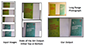
\includegraphics[width=1cm]{figures/teaserThumbail.png} in the paper.
One can immediately observe that the quadcopter is flying autonomously; the control of the quadcopter,
especially in outdoor environment, is a difficult problem but is unrelated to the computer vision task
discussed in this paper.

\hrule
\href{videos/lady1.avi} {Video} related to Figure
7~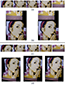
\includegraphics[width=1cm]{figures/lady1Thumbail.png} in main paper.

\hrule

\href{videos/greenRed.avi} {Video} related to Figure
8~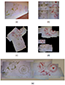
\includegraphics[width=1cm]{figures/greenRedThumbail.png} in main paper.

\hrule
This section contains an additional result, i.e., an entry not in the main paper.  We want to emphasize that we have performed several experiments,
and this is yet another example.  
%We are not including all ``new" examples.
% SC Your latex citation is not appearing (see Autostitch in the caption
% MGP Done
% SC set figure caption value to be a number more than the last figure in the main paper
% SC so that there is no confusion between this FIgure 1 and the Figure 1 in the main paper
% MGP Done


The input \href{videos/lady2.avi}{stream} had about 9000 images. The
selection algorithm of Section 3 pruned the video into $N=15$ images. The scene as captured by a typical camera 
can  be seen in
Figure~\ref{fig:validResults}(a). A sample of the
selected images are seen in Figure~\ref{fig:validResults}(b).
Figure~\ref{fig:validResults}(c,d,e) shows the comparison of outputs of the state
of the art stitching methods with the output of our algorithm. The input videos
are such that there are no vacant
spaces; our stitching algorithm's output is similar to that of Autostitch
\cite{autostitch} as well as Photoshop \cite{photoshop}.


\begin{figure*}[h!]
\centering
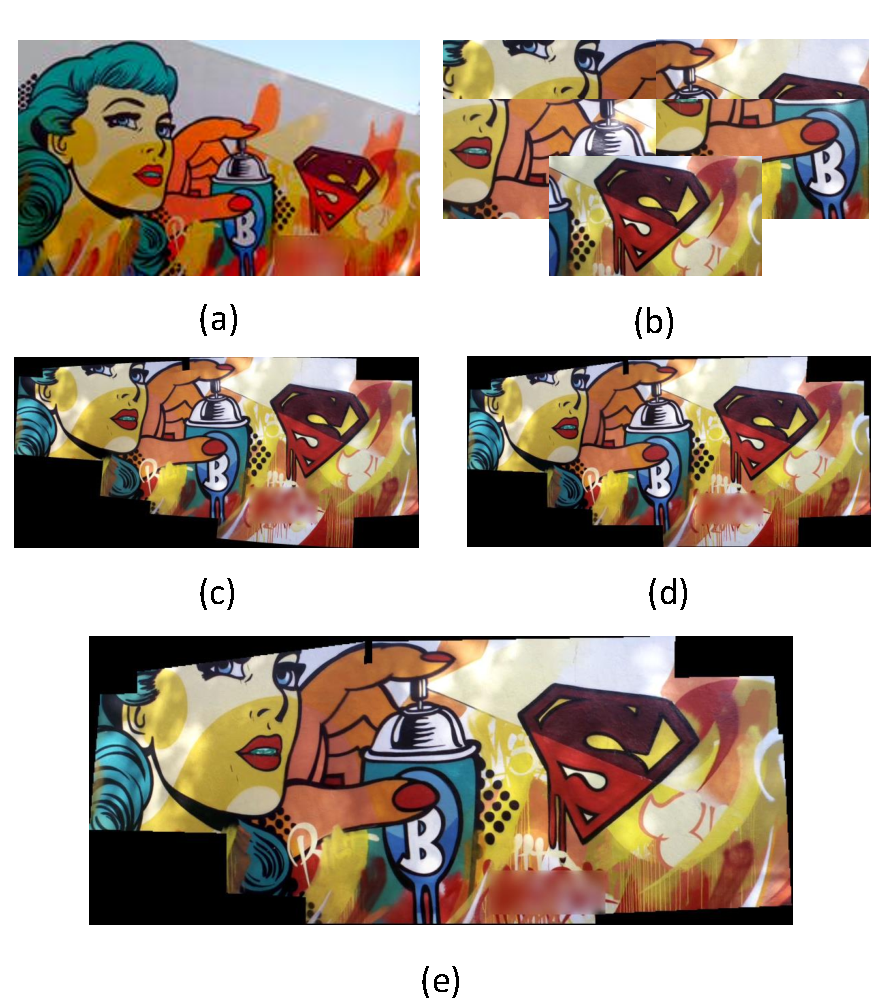
\includegraphics[width=0.87\linewidth]{figures/lady2.pdf}
\caption{ (a) Uniformly sampled images from an outdoor video
  expedition.  (b) Salient image selection from the set of
  approximately 9000 images using positional information. (c) Output from
  Autostitch \cite{autostitch} (d) Output from Adobe Photoshop CS6
  \cite{photoshop} output (e) Output from this paper.}
\label{fig:validResults}
\end{figure*}

\hrule
% 
% \begin{figure*}[h!]
% \centering
% 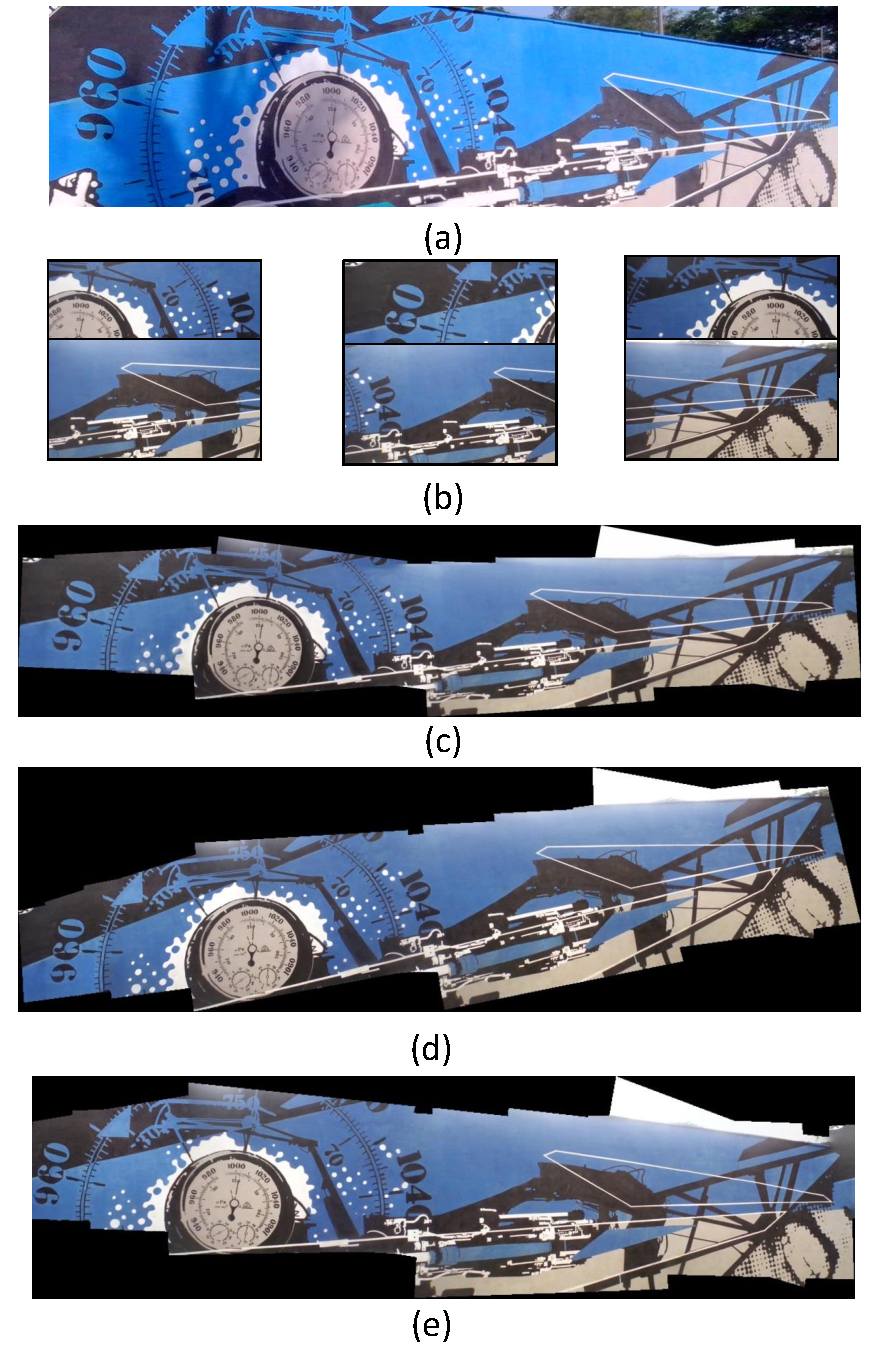
\includegraphics[width=0.8\linewidth]{figures/longwall.pdf}
% \caption{ (a) Uniformly sampled images from an outdoor video
%   expedition.  (b) Salient image selection from the set of
%   approximately 9000 images using positional information. (c) Autostitch output
%   (d) Adobe Photoshop CS6 output (e) Our output }
% \label{fig:validResults1}
% \end{figure*}
% 
% The input \href{videos/longwall.avi}{stream} had about 4000 images. The
% selection algorithm pruned the video into $N=19$ images.
% The scene as captured by a typical camera  can also be seen in
% Figure~\ref{fig:validResults1}(a). A sample of the
% selected images are seen in Figure~\ref{fig:validResults1}(b).
% Figure~\ref{fig:validResults1}(c,d,e) shows the comparison of outputs of state
% of the art stitchers with the output of our algorithm. As there are no vacant
% spaces, our stitching algorithm's output is similar to that of Autostitch as
% well as Photoshop.

\begin{figure*}[h!]
\centering
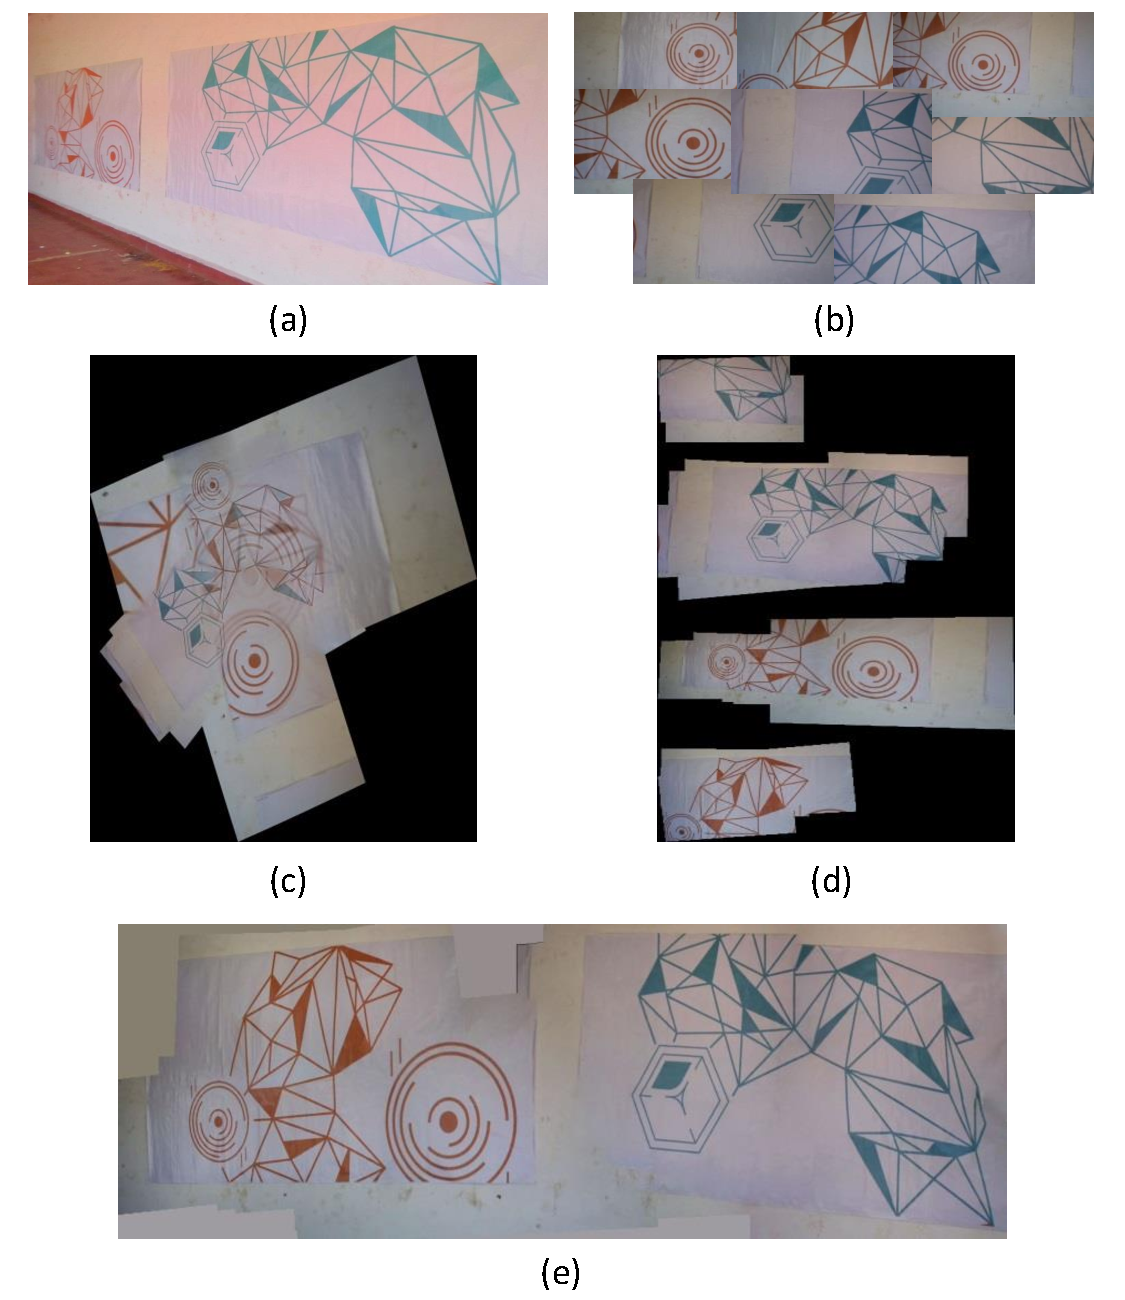
\includegraphics[width=0.85\linewidth]{figures/orange_blue.pdf}
\caption{(a) An outdoor scene captured by a standard camera in an
  exhibition. The approach to the area is normally cordoned off and one
  needs permission to get a quadcopter to take the picture.  Notice a
  significant gap between the two posters.  (b) Pruned images from the
  quadcopter video using our saliency algorithm. (c) Output of
  Autostitch~\cite{autostitch} on the selected images. The mosaic is not
  reasonable presumably because of the confusion in features. (d) Output of Adobe
  Photoshop CS6~\cite{photoshop} on the selected images. The vacant space posed
  a problem to the feature matching algorithm, so instead of a mosaic,
  individual pieces were output as mini-panoramas (e) Our output on
  the selected images. We are able to join two posters (separated by
  vacant space) using IMU data.}
\label{fig:results1}
\end{figure*}

The input \href{videos/orangeBlue.avi}{stream} had about 9100 images. The
selection algorithm pruned the video into $N=28$ images. The scene as captured by a smartphone can also be seen in
Figure~\ref{fig:results1}(a). A sample of the
selected images are seen in Figure~\ref{fig:results1}(b).
Figure~\ref{fig:results1}(c,d,e) shows the comparison of outputs of state
of the art stitchers with the output of our algorithm. As there are vacant
spaces, Autostitch~\cite{autostitch} as well as Photoshop~\cite{photoshop} are
unable to stitch images accurately. In contrast, since we use positional data, our output is an acceptable mosaic, and shows
an orthographic view. 

\hrule
\begin{figure*}[h!]
\centering
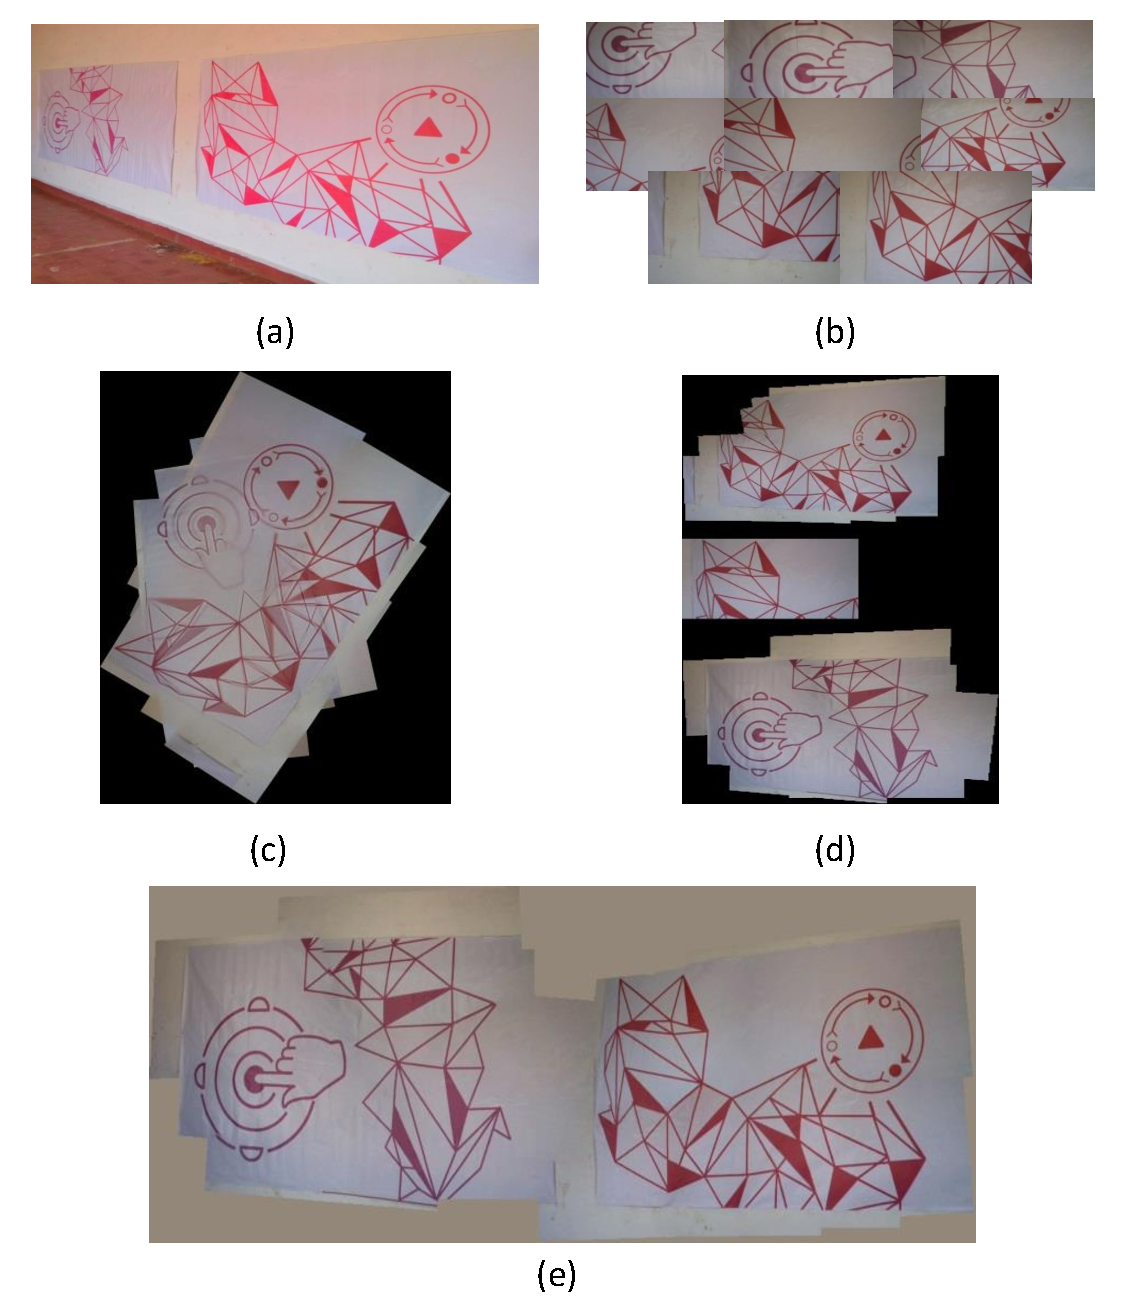
\includegraphics[width=0.85\linewidth]{figures/Purple_red.pdf}
\caption{(a) An outdoor scene captured by a standard camera in an
  exhibition. Notice a   significant gap between the two posters.  (b) Pruned
  images from the quadcopter video using our saliency algorithm. (c) Output of
  Autostitch~\cite{autostitch} on the selected images. The mosaic is not
  reasonable presumably because of the confusion in features. (d) Output of Adobe
  Photoshop CS6~\cite{photoshop} on the selected images. The vacant space posed a
  problem to the feature matching algorithm, so instead of a mosaic,
  individual pieces were output as mini-panoramas (e) Our output on
  the selected images. We are able to join two posters (separated by
  vacant space) using IMU data.}
\label{fig:results2}
\end{figure*}
	
The input \href{videos/purpleRed.avi}{stream} had about 8500 images. The
selection algorithm pruned the video into $N=17$ images.The scene as captured by a smartphone can also be seen in
Figure~\ref{fig:results2}(a). A sample of the
selected images are seen in Figure~\ref{fig:results2}(b).
Figure~\ref{fig:results2}(c,d,e) shows the comparison of outputs of state
of the art stitchers with the output of our algorithm. As there are vacant
spaces, Autostitch~\cite{autostitch} as well as Photoshop~\cite{photoshop} are
not able to stitch images accurately. But, as we are using IMU data, our output is closest to input scene.
	
\bibliographystyle{ieee}
\bibliography{egbib}	
\end{document}